\documentclass[11pt,a4paper]{article}
\usepackage[paperwidth=210mm,paperheight=440mm,margin=1.5cm]{geometry}
\usepackage{graphicx}
\usepackage{float}
\usepackage{caption}
\usepackage{subcaption}
\usepackage{amsmath}
\usepackage[hidelinks]{hyperref}
\usepackage{xcolor}

% No page numbers
\pagestyle{empty}
\makeatletter
\let\ps@plain\ps@empty
\makeatother

\setlength{\parindent}{0pt}
\setlength{\parskip}{0.5em}
\captionsetup{font=small,labelfont=bf}

\newcommand{\resultpair}[5]{%
\begin{figure}[H]
    \centering
    \begin{subfigure}[t]{0.48\linewidth}
        \centering
        \includegraphics[width=\linewidth]{../results/#1}
        \caption{#2}
    \end{subfigure}
    \hfill
    \begin{subfigure}[t]{0.48\linewidth}
        \centering
        \includegraphics[width=\linewidth]{../results/#3}
        \caption{#4}
    \end{subfigure}
    \caption{#5}
\end{figure}
}

\title{Diffusion Exercise: MNIST Digit Generation}
\author{}
\date{}

\begin{document}

\maketitle

This report shows the results from training a DDPM on the MNIST handwritten digit dataset...
and I've just about had it with this exercise...



\section*{Training Curve}

\begin{figure}[H]
    \centering
    
\includegraphics[width=0.72\linewidth]{../results/loss_curve.png}
    \caption{Training loss during the DDPM run.}
    \label{fig:loss-curve}
\end{figure}

\section*{Generated Samples During Training}

\begin{figure}[H]
    \centering

    \begin{subfigure}{0.30\linewidth}
        \centering
        
\includegraphics[width=\linewidth]{../results/samples_before_training.png}
        \caption{Before training}
    \end{subfigure}
    \begin{subfigure}{0.30\linewidth}
        \centering
        
\includegraphics[width=\linewidth]{../results/samples_epoch_10.png}
        \caption{10 epochs}
    \end{subfigure}
    \begin{subfigure}{0.30\linewidth}
        \centering
        
\includegraphics[width=\linewidth]{../results/samples_epoch_20.png}
        \caption{20 epochs}
    \end{subfigure}

    \begin{subfigure}{0.30\linewidth}
        \centering
        
\includegraphics[width=\linewidth]{../results/samples_epoch_30.png}
        \caption{30 epochs}
    \end{subfigure}
    \begin{subfigure}{0.30\linewidth}
        \centering
        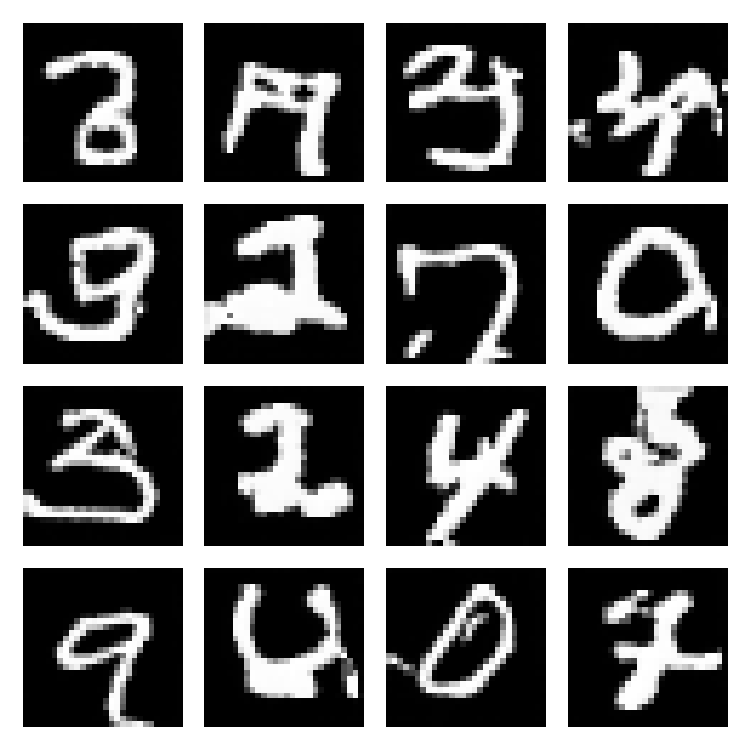
\includegraphics[width=\linewidth]{../results/samples_epoch_40.png}
        \caption{40 epochs}
    \end{subfigure}
    \begin{subfigure}{0.30\linewidth}
        \centering
        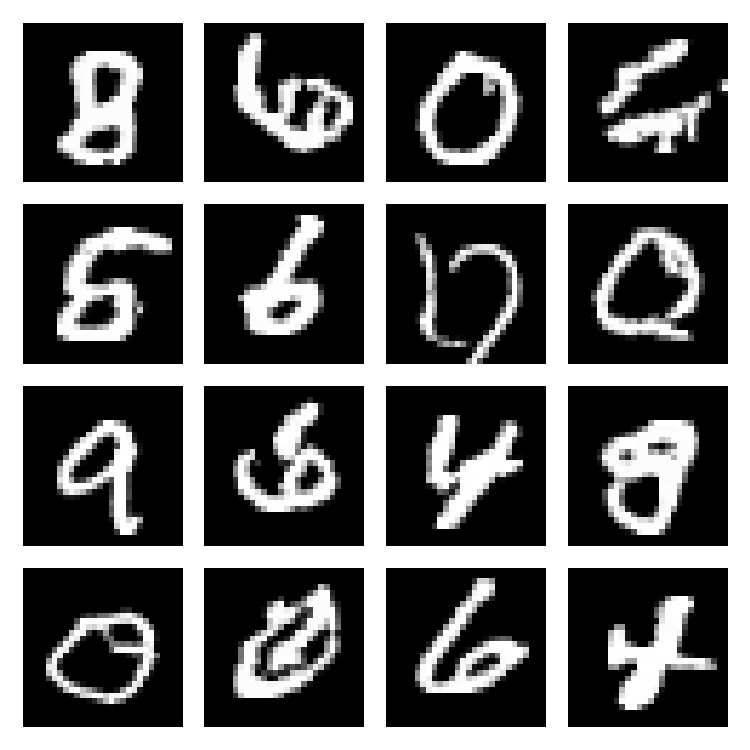
\includegraphics[width=\linewidth]{../results/samples_epoch_50.png}
        \caption{50 epochs}
    \end{subfigure}

    \caption{Generated samples...}
    \label{fig:samples-training}
\end{figure}

\end{document}
